%!TEX root = ../NCVC7.tex
\mysection{荒加工用のNCデータを生成}

\subsection{IGESデータの読み込み}
 図~\ref{fig:sample.iges} のIGESデータをNCVCで読み込みます.
この時点で \ref{sec:AboutIGES}節にも書いたようにNCVCが落ちる場合があります.
IGESタイプを変更するなど適宜対応してください.

\begin{figure}[H]
\centering
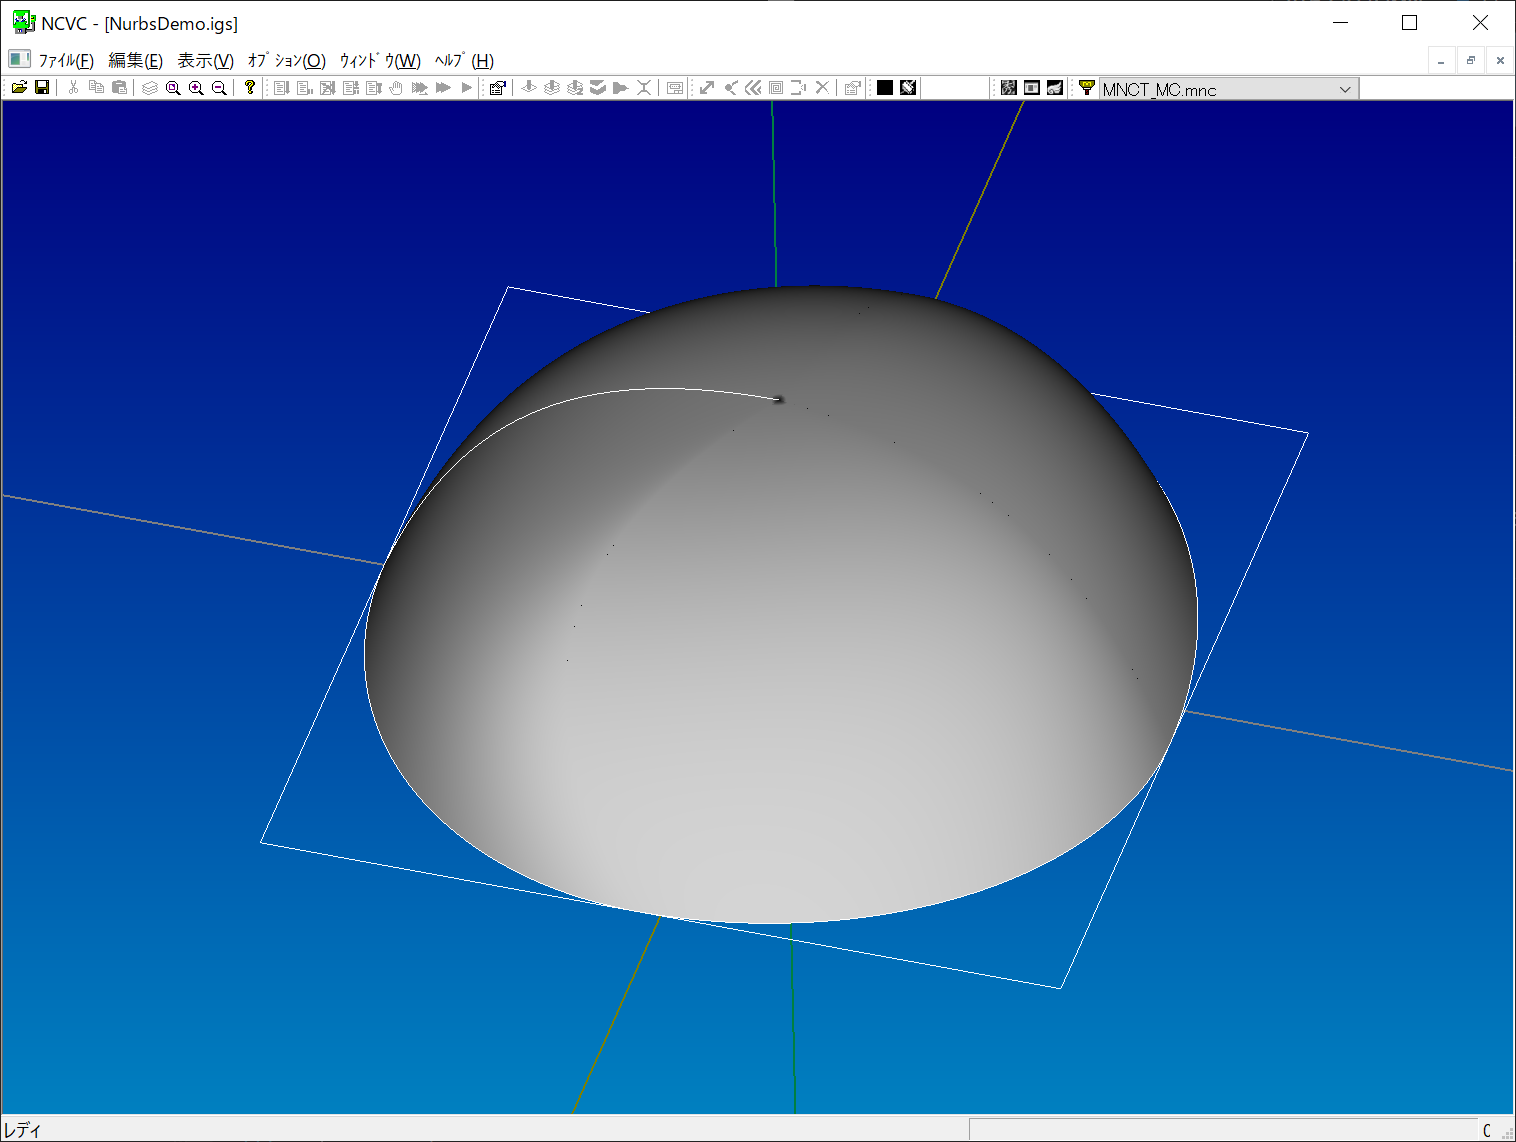
\includegraphics[scale=0.5]{No2/fig/fig21.png}
\caption{サンプル図形の読み込み}
\label{fig:ncvc21}
\end{figure}

 なお,\textbf{IGESデータと同じ場所に設定用のファイル(~.ncvc)が自動的に作られます.}
インストーラ付属のサンプルデータを使用する場合は,ドキュメントフォルダ等の書き込み権限がある場所にコピーしてから使用してください.

\subsection{荒加工用スキャニングパスの生成}
 荒加工用のデータを生成するには,切削対象となる1つのNURBS曲面と,ガイドとなる1つのNURBS曲線を選択する必要があります.
マウスの左クリックで選択してください.選択順は問いません.
選択できると選択色
\footnote{\menu{オプション>表示属性>表示属性の設定}から\menu{共通}タブの\menu{選択オブジェクト}の色}
に変わります.

\begin{figure}[H]
\centering
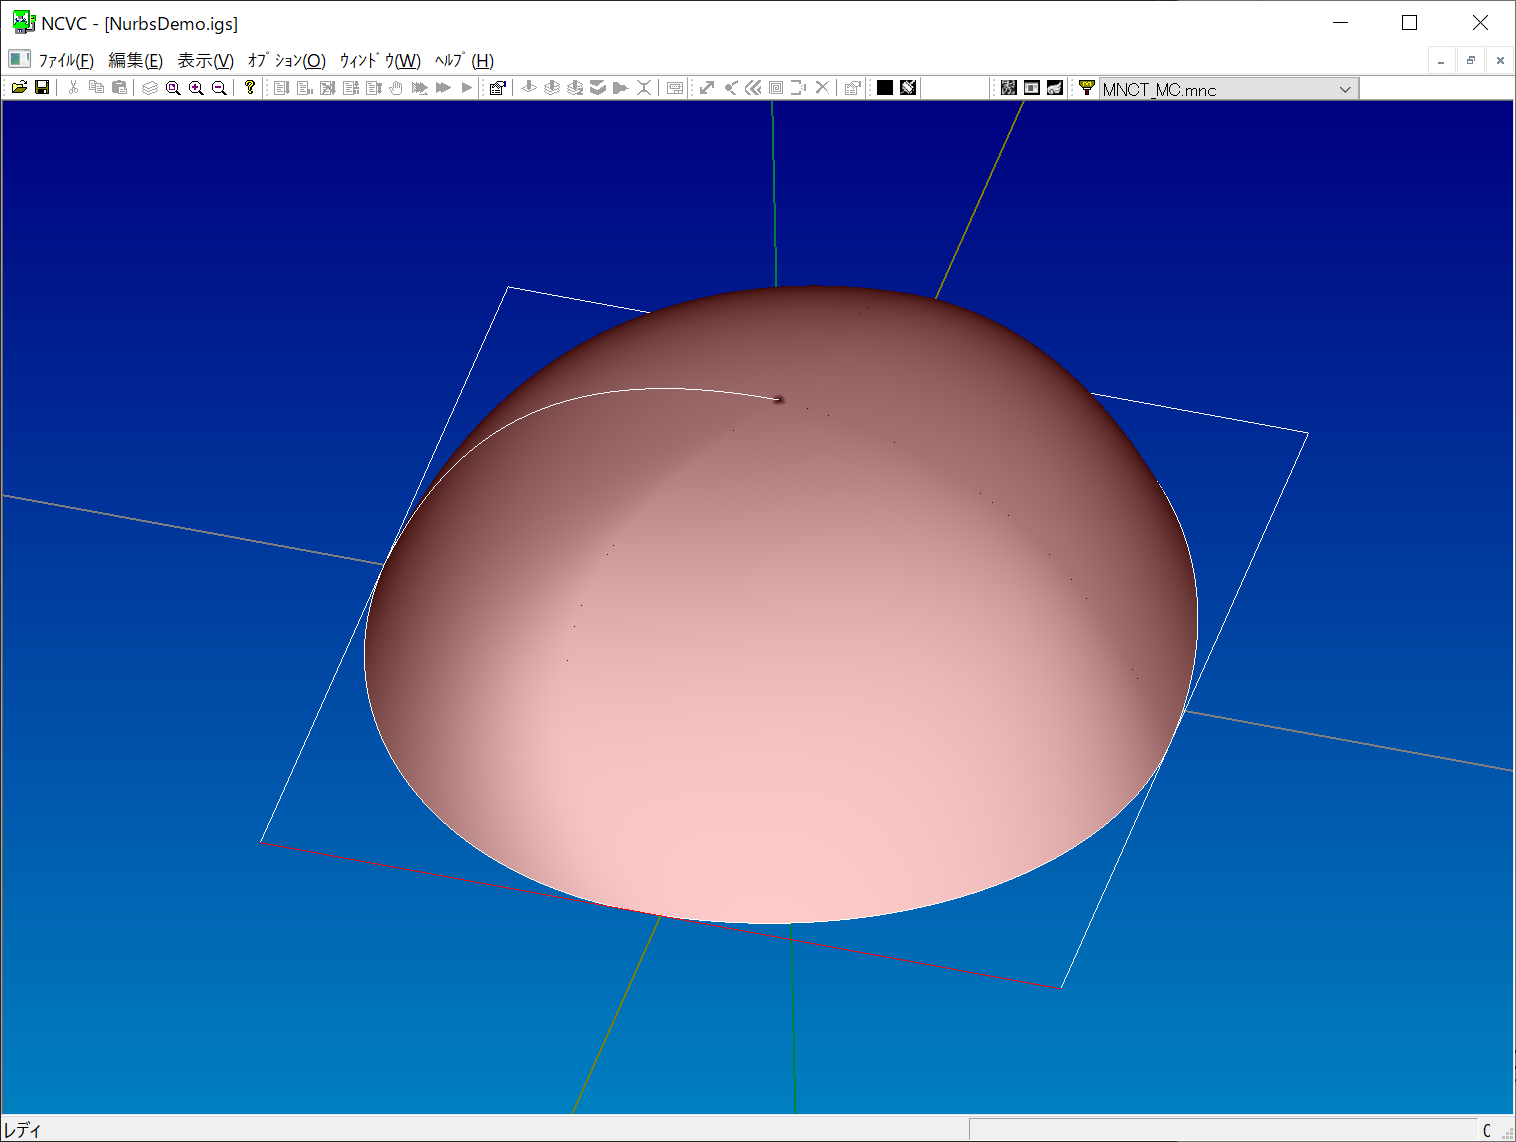
\includegraphics[scale=0.5]{No2/fig/fig22.png}
\caption{NURBS曲面とNURBS曲線の選択}
\label{fig:ncvc22}
\end{figure}

 NURBS曲面とNURBS曲線を選択すると,\menu{ファイル>NCデータの生成>荒加工パスの生成}メニュー(\keys{F2})が有効になります.
適当な値を設定してください.

 [NC生成時,ワーク上面をZ軸のゼロにする]にチェックが入っていると[ワークの高さ]で設定した高さがZ軸のゼロになるようにNCデータが生成されます.
通常はチェックを入れておきましょう.

\begin{figure}[H]
\centering
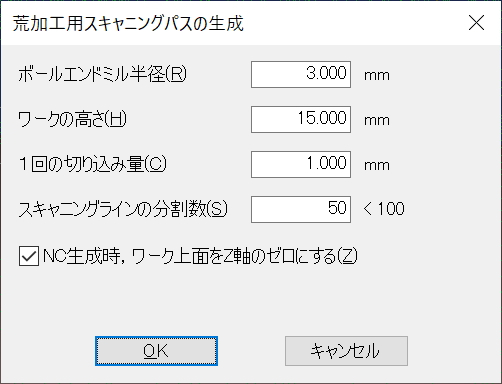
\includegraphics{No2/fig/fig23.png}
\caption{荒加工スキャニング設定}
\label{fig:ncvc23}
\end{figure}

 図~\ref{fig:ncvc23} で \keys{OK} を押すと,しばらく計算したあと,図~\ref{fig:ncvc24} のように荒加工パスが表示されます.
選択されたガイド曲線が[スキャニングラインの分割数]で分割され,さらにそのガイド曲線に沿うように点群が生成されます.

\begin{figure}[H]
\centering
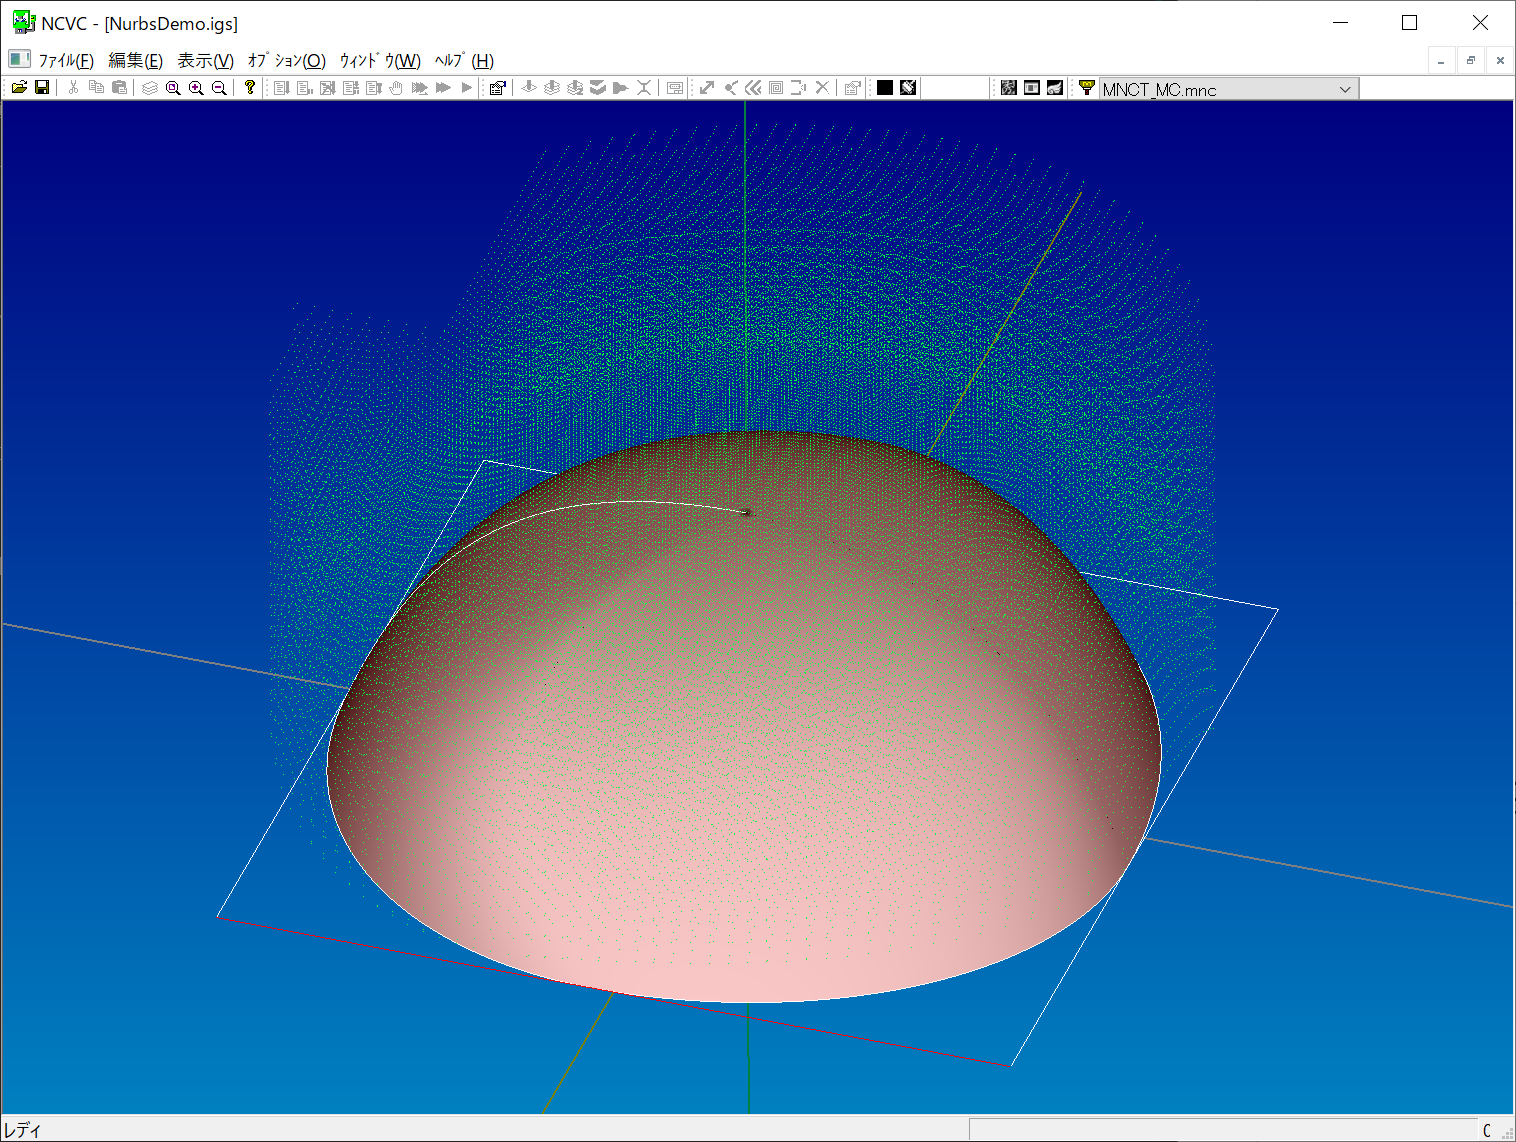
\includegraphics[scale=0.5]{No2/fig/fig24.png}
\caption{荒加工スキャニングパスの表示Ⅰ}
\label{fig:ncvc24}
\end{figure}

 図~\ref{fig:ncvc22} ではモデルの手前にあるX軸と平行なガイド曲線を選択したので,点群は図~\ref{fig:ncvc24} のようにY方向の集まりになりますが,
ガイド曲線をモデルの右(または左)側にあるY軸と平行なガイド曲線を選択すると,図~\ref{fig:ncvc25} のように点群はX方向の集まりになります.
\textbf{どちら方向に切削するかは,このガイド曲線の選択によって変わります.}

\begin{figure}[H]
\centering
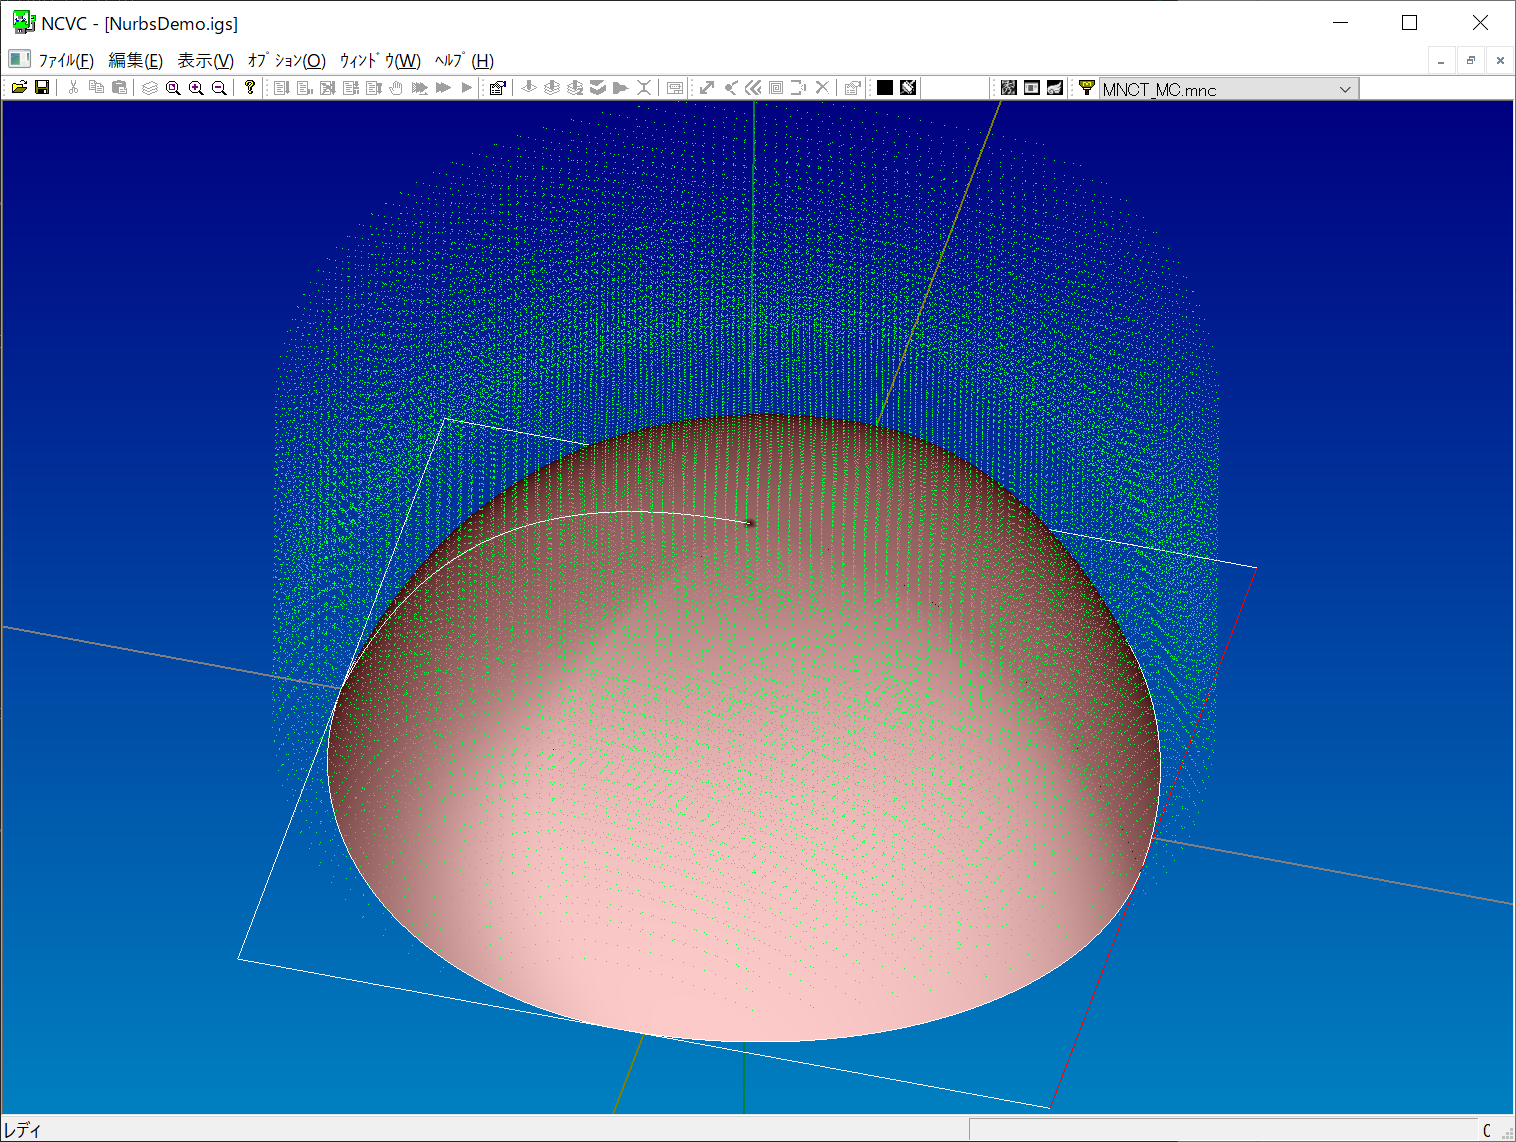
\includegraphics[scale=0.5]{No2/fig/fig25.png}
\caption{荒加工スキャニングパスの表示Ⅱ}
\label{fig:ncvc25}
\end{figure}
